\documentclass[12pt]{article}

\usepackage{answers}
\usepackage{setspace}
\usepackage{graphicx}
\usepackage{enumitem}
\usepackage{multicol}
\usepackage{mathrsfs}
\usepackage[margin=1in]{geometry} 
\usepackage{amsmath,amsthm,amssymb,mathtools}
\usepackage{titlesec}

\newcommand\numberthis{\addtocounter{equation}{1}\tag{\theequation}}

\titleformat{\section}[runin]{\normalfont\Large\bfseries}{\thesection}{1em}{}
\titleformat{\subsection}[runin]{\normalfont\large\bfseries}{\thesubsection}{1em}{}

\def\tf{\textbf}
\def\tt{\textit}
\def\mc{\ensuremath\mathcal}
\def\mf{\ensuremath\mathbf}
\def\mt{\ensuremath\mathit}
\def\mb{\ensuremath\mathbb}
\def\td{\ensuremath\tilde}
\def\N{\ensuremath\mb{N}}
\def\Z{\ensuremath\mb{Z}}
\def\C{\ensuremath\mb{C}}
\def\R{\ensuremath\mb{R}}
\def\S{\ensuremath\mb{S}}
\def\V{\ensuremath\mb{V}}
\def\W{\ensuremath\mb{W}}
\def\Ber{\ensuremath\mf{Ber}}
\def\det{\ensuremath\mf{det}}
\def\sigm{\ensuremath\mf{sigm}}
\def\diag{\ensuremath\mf{diag}}
\def\dom{\ensuremath\mf{dom}}
\def\cond{\ensuremath\mf{cond}}
\def\sign{\ensuremath\mf{sign}}
\def\bd{\ensuremath\mf{bd}}
\def\rto{\ensuremath\rightarrow\ }
\def\Rto{\ensuremath\Rightarrow\ }
\def\lto{\ensuremath\leftarrow\ }
\def\Lto{\ensuremath\Leftarrow\ }
\def\xrto{\ensuremath\xrightarrow}
\def\xRto{\ensuremath\xRightarrow}
\def\xlto{\ensuremath\xleftarrow}
\def\xLto{\ensuremath\xLeftarrow}
\def\rvec{\ensuremath\overrightarrow}
\def\lvec{\ensuremath\overleftarrow}

\providecommand\P[1]{}
\renewcommand\P[1]{\mb{P}\{#1\}}
\providecommand\E[1]{}
\renewcommand\E[1]{\mb{E}[#1]}
\providecommand\Var[1]{}
\renewcommand\Var[1]{\mf{Var}(#1)}
\providecommand\p[2]{}
\renewcommand\p[2]{\frac{\partial #1}{\partial #2}}
\providecommand\pp[2]{}
\renewcommand\pp[2]{\frac{\partial^2 #1}{\partial #2^2}}
\providecommand\ps[3]{}
\renewcommand\ps[3]{\frac{\partial^2 #1}{\partial #2\partial #3}}
\providecommand\d[2]{}
\renewcommand\d[2]{\frac{d #1}{d #2}}

\DeclareMathOperator{\sech}{sech}
\DeclareMathOperator{\csch}{csch}
    
\begin{document}
    
\title{Non-Euclidean Geometry - Notes}
\author{Dhruv Kohli}
\maketitle
\section{Introduction}
\begin{itemize}
    \item Parallel Axiom: Through any point $p$ not on the line $L$ there exists precisely one line $L'$ that does not meet $L$. This axiom cannot be practically tested.

    \item Girolamo Saccheri in $1733$ proposed that if Parallel Axiom is not true then two alternatives will arise:
    \begin{itemize}
        \item Spherical Axiom. There is no line through $p$ that does not meet $L$. Naming of this will become clear. Saccheri obtained contradiction provided "lines" are assumed to have infinite length. If this cannot be assumed then one obtain a NEG called SG.

        \item Hyperbolic Axiom. There are atleast two lines through $p$ that do not meet $L$. Name of this is obscure but standard. No contradiction could be attained, yielding another NEG called HG.
    \end{itemize}

    \begin{figure}[h!]
        \centering
        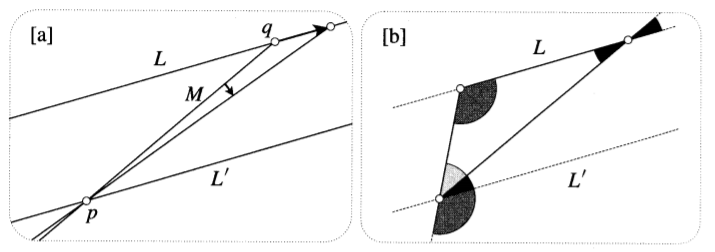
\includegraphics[scale=0.7]{fig_1}
        \label{fig_1}
    \end{figure}

    \item A theorem in EG is that: angle sum of any triangle is $\pi$. This result is actually equivalent to parallel axiom. In NEG the angle sum of a triangle differs from $\pi$. Angular excess $E(T) \equiv \sum\angle(T) - \pi$. EG is characterized by vanishing $E(T)$. Unlike parallel axiom, this statement can be checked against experiment. Gauss and Johann Heinrich Lambert independently discovered that,
    \begin{itemize}
        \item In SG, $E(T) > 0$.

        \item In HG, $E(T) < 0$.
    \end{itemize}
    They also discovered that $E(T)$ is completely determined by the size of the triangle i.e. $E(T) \propto A(T)$ and $E(T)=kA(T)$ where $k$ is a constant that is $>0$ for SG and $<0$ for HG.
    \begin{itemize}
        \item Although there are no qualitative differences between them, there are infinitely many different spherical and hyperbolic geometries depending on the constant $k$.

        \item Since $\sum\angle(T)$ cannot be negative $E(T) \geq -\pi$. Thus in HG no triangle can have area greater than $|\pi/k|$.

        \item In NEG, similar triangles do not exist because $E(T)$ for two triangles of different areas will be different.

        \item In NEG, there exist an absolute unit of length. For example, in SG we could define it to be the side of equilateral triangle having $\sum\angle(T) = 1.01\pi$ and in HG, to be the side of equilateral triangle having $\sum\angle(T)=0.99\pi$.

        \item More natural way of defining the absolute unit of length is in terms of constant $k$. Since, $E(T)$ is a number, $k$ has units of $1/(\text{length}^2)$, so, it can be written in terms of a length $R$: $k=+(1/R^2)$ in SG and $k=-(1/R^2)$ in HG.

        \item The smaller the triangle, the harder it is to distinguisg it from a Euclidean triangle: only when the linear dimensions are a significant fraction of $R$ will the difference become obvious.
    \end{itemize}

    \item Gauss never published his ideas on NEG. Janos Bolyai (1832) and Nikolai Lobachevsky (1829) independently discovered HG but their work was ignored. Eugenio Beltrami in 1868 discovered pseudosphere s.t. figures drawn on it automatically obey rules of HG.

    \item Geodesic: Shortest route connecting two points on a curved surface. The distance between $a$ and $b$ on a curved surface is the length of the geodesic segment connecting them.

    \item It is the curvature of the surface that causes $E(T)$ to differ from $0$. However, it cannot be the precise shape of the surface in space that is involved here.

    \item Stretch-free bending changes extrinsic geometry but does not change intrinsic geometry (an intelligent ant living on the surface would not find any change in the shortest distance between two points on surface). Also, value of $E$ is unaffected by stretch-free bending (because shortest distances are same). So, $E$ is governed by intrinsic (not extrinsic) curvature.

    \item Gaussian curvature $k(p)$ which quantifies the amount and type of bending of the surface at a point $p$ is defined as follows. Let $\prod$ be a plane containing normal vector $\mf{n}$ to the surface at $p$, and $\kappa$ be the signed curvature at $p$ of the curve in which $\prod$ intersects the surface. The sign of $\kappa$ depends on whether the centre of curvature is in the direction $\mf{n}$ or $-\mf{n}$. The so-called principal curvatures are the minimum $\kappa_{min}$ and $\kappa_{max}$ values of $\kappa$ as $\prod$ rotates about $\mf{n}$ (Euler previously made the discovery that these principal curvatures occur in perpendicular directions). Gauss defined $k(p)$ as product $\kappa_{min}\kappa_{max}$. Higher the magnitude of $k(p)$ higher then bending at $p$. Sign of $k(p)$ determines the type of bending where positive sign corresponds to spherical bending while negative sign correspnds to hyperbolic (saddle like) bending. Note that $k(p)$ is calculated using extrinsic geometry of the surface but Gauss discovered that it actually computes the intrinsic curvature of the surface at $p$ i.e. $k$ is invariant under stretch-free bending (Gauss called this Theorema Egregium (remarkable theorem)).

    \begin{figure}[h!]
        \centering
        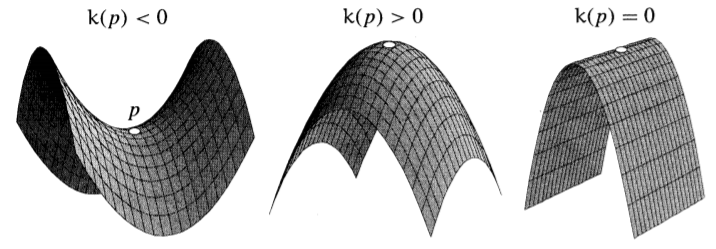
\includegraphics[scale=0.7]{fig_2}
        \label{fig_2}
    \end{figure}

    \item It is easy to see viusally that $k(p)=0$ everywhere on a flat surface. The intrinsic significance of $k(p)$ is exhibited in the following result: If $\Delta$ is an infinitesimal triangle of area $dA$ located at $p$, then $E(\Delta) = k(p)dA$ (proof in differential geometry). Since $E$ and $dA$ are defined by intrinsic geometry, so is $k(p) = (E/dA)$. So, angular excess of a triangle $T$ is obtained by adding up the Gaussian curvature over the interior of $T$: $E(T) = \int\int_{T}k(p)dA$.

    \item A surface of constant curvature is the one which has same value of $k(p)$ for all $p$ on surface. For example: a plane has $k(p)=0$ for all $p$, a sphere has $k(p)=1/R^2$ for all $p$ and a pseudosphere has $k(p)=-1/R^2$ for all $p$. Also, $E(T) = kA(T)$ for a constant curvature surface. This is identical to fundamental formula of NEG. As Beltrami realized, E, S and H G can all be interpretd concretely as the intrinsic geometry of surfaces of constant vanishing, positive or negative curvature.

    \item The requirement of constant curvature can be understood more intuitively as follows. In EG, two figures are congruent if there exist a motion that carries the first into coincidence with second. For this basic concept of equality be available in NEG, we require that our surface admits an analogous group of motions. But, variation in the curvature is the obstruction to motion (remember that we are concerned with motion corresponding to stretch-free bending). Clarification between constant curvature and the existence of motions: Consider infinitesimal (bendable but unstretchable) triangle located at $p$. If its angular excess is $E$ and its area is $dA$ then Gaussian curvature at $p$ is $E/d(A)$. Now, suppose that there exist a motion that carries this traingle to another arbitrary points $q$ on the surface. We may have to bend the triangle to fit it but since it is not stretched, $E$ and $dA$ does not change. So, $k(q)=E/dA=k(p)$ and the surface has constant curvature.

    \item If the Euclidean plane is identified with $\C$ then its motions (and similarities) are represented by M.T. $M(z)=az+b$. Motions of SG and HG are also M.T. The most general (direct) motion of the sphere is a rotation about its centre. Stereographic projection onto $\C$ yields a conformal map of the sphere to the complex plane, and the rotations of the sphere thus become complex functions acting on this map. As we showed in earlier chapter, they are M.T. of the form $(az+b)/(-\bar{b}z+\bar{a})$. This was first discovered by Gauss in 1819. It is also possible to construct conformal maps in $\C$ of the pseudosphere, thereby transforming its motions into complex functions. One of the most convenient of these conformal maps is constructed in the unit disc. The motions of HG then turn out to be the M.A. of this circular map: $(az+b)/(\bar{b}z+\bar{a})$. This discovery was made by Poincare. We will also learn that most general mobius transformation $(az+b)/(cz+d)$ represents the most general (direct) motion of the three dimensional hyperbolic space.
\end{itemize}
\section{Spherical Geometry}
\begin{itemize}
    \item Geodesics on the sphere are great circles, that is the intersections of the sphere with planes through its centre. These are called lines in SG.

    \item Angular excess of a spherical triangle: $A(T) + A(T_a) + A(T_b) + A(T_c) = 4\pi R^2/2 = 2\pi R^2$. Also, $A(T) + A(T_a) = 2aR^2$, $A(T) + A(T_b) = 2bR^2$ and $A(T) + A(T_c) = 2cR^2$. Solving these equations we get, $2A(T) = 2(\alpha+\beta+\gamma-\pi)R^2$ so that $A(T) = E(T)R^2$ and $E(T) = A(T)/R^2$. So, $k=1/R^2$.

    \begin{figure}[h!]
        \centering
        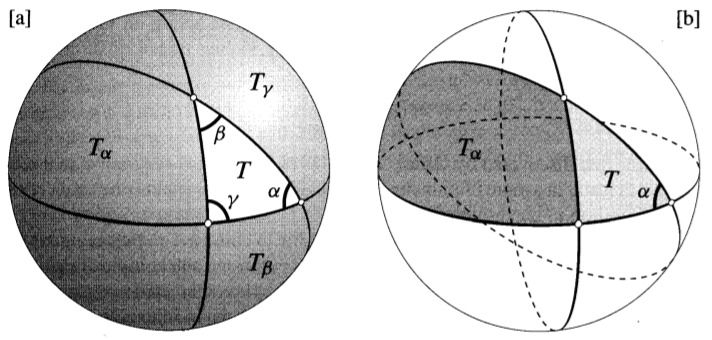
\includegraphics[scale=0.7]{fig_3}
        \label{fig_3}
    \end{figure}

    \item Distance between two points $a$ and $b$ on a sphere is defined to be the length of the shorter arc of the great circle (line) passing through the two points. Note that length is $\pi R$ when $a$ and $b$ are antipodal.
    
    \item As for a plane, motion of sphere is uniquely determined by images $a',b',c'$ of three points $a,b,c$ not on a line (note that the image of a point $P$ is the unique point $P'$ whose distances from $a',b',c'$ equal the distances of $P$ from $a,b,c$).
    
    \item By convention, an angle is positive if it is counter-clockwise when viewed from outside the sphere. As for a plane, spherical motions can thus be divided into two types: direct (i.e. conformal) motions and opposite (i.e. anticonformal) motions.
    
    \item As in the plane, the simplest opposite motion of sphere is reflection in a line (great circle) $L$. This may be thought of as reflection of the space in the plane $\prod$ containing $L$. To reflect $a$ in $L$, draw a line $M$ through $a$ that intersects $L$ at right angles. If $d$ is the distance of $a$ from the point of intersection then reflection of $a$ in $L$ is the point obtained after walking a further distance $d$ from point of intersection. Depending on the direction of walk, there can be two values of $d$, however, both will give same result as long as we travel in the same direction as we walked before.

    \begin{figure}[h!]
        \centering
        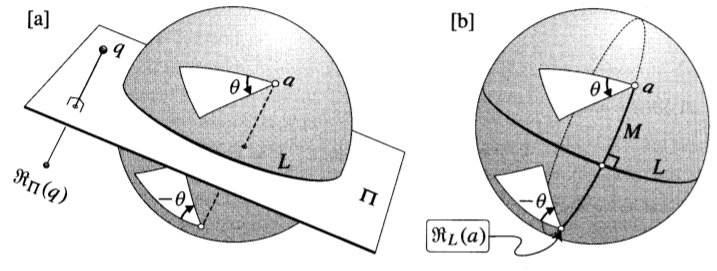
\includegraphics[scale=0.7]{fig_4}
        \label{fig_4}
    \end{figure}

    \item Rotation of sphere about an axis $V$ passing through its centre is clearly a direct motion (these are the only direction motions of the sphere will proved later). This rotation could be denoted by $R^{\theta}_{p}$ which is rotation of $\theta$ in counter-clockwise direction as $p$ is seen from outside about axis passing through $p$ and its antipodal point $q$. Note that $R^{\theta}_{p} = R^{-\theta}_{q}$.
    
    \item In a plane, all direct motions are compositon of two reflections. On a sphere, compositon of two reflections in two lines (great circles) results in rotation of above type. Note that two lines on sphere always intersect so there is no motion analogous to translation for a sphere.
    
    \begin{figure}[h!]
        \centering
        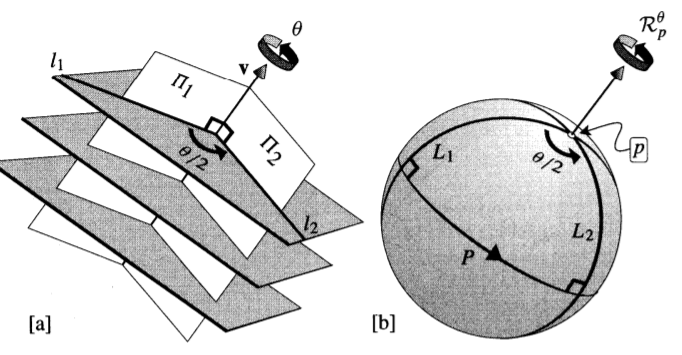
\includegraphics[scale=0.7]{fig_5}
        \label{fig_5}
    \end{figure}

    \item As in the figure, $\mc{R}_{L_2}\circ \mc{R}_{L_1} = R_{p}^{\theta}$. So a rotation $R^{\theta}_{p}$ of the sphere about a point $p$ through angle $\theta$ may be expressed as the compositon of reflections in any two spherical lines that pass through $p$ and contain the angle $\theta/2$.
    
    \item There is exactly one line $P$ that is mapped to itself by $R^{\theta}_{p}$. It is called polar line of $p$ and $p$ is called pole of $P$.

    \begin{figure}[h!]
        \centering
        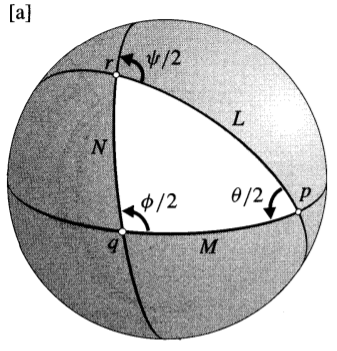
\includegraphics[scale=0.7]{fig_6}
        \label{fig_6}
    \end{figure}
    
    \item The composition of any two rotations of the sphere is equivalent to a single rotation. Thus the set of all rotations of the sphere forms a group. As in figure, $R^{\phi}_{q}\circ R^{\theta}_{p} = (\mc{R}_{N} \circ \mc{R}_{M}) \circ (\mc{R}_{M} \circ \mc{R}_{L}) = \mc{R}_{N} \circ \mc{R}_{L} = R_{r}^{\psi}$. Note that in contrast to plane where $\psi = \phi+\theta$, for sphere, $\psi/2 = \theta/2+\phi/2-kA(T)$ so that $\psi = \theta+\phi-2kA(T)$.

    \begin{figure}[h!]
        \centering
        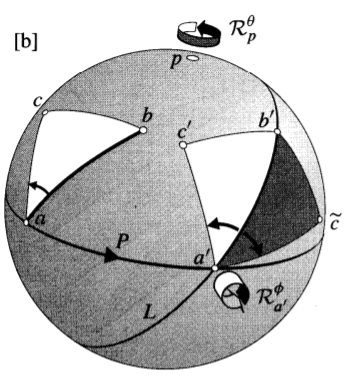
\includegraphics[scale=0.7]{fig_7}
        \label{fig_7}
    \end{figure}
    
    \item There is exactly one direction motion $\mc{M}$ and exactly one opposite motions $\td{\mc{M}}$ that maps a given line segment $ab$ to another line segment $a'b'$ of equal length. Furthermore, $\td{\mc{M}}=\mc{R}_{L}\circ \mc{M}$ where $L$ is the line through $a'$ and $b'$. As in figure, $\mc{M} = R_{a'}^{\phi} \circ R_{p}^{\theta}$ which is equivalent to a single rotation. So, every direct motion of the sphere is a rotation and every opposite motion is the composition of a rotation and a reflection.
    
    \item Antipodal mapping that sends every point on sphere to its antipodal point is a motion (preserves distances). This can be realized by rotation of $\pi$ about an axis formed by two antipodal points $p$ and $q$ and then taking reflection in line passing through these two points. It is an opposite motion.

    \item The knowledge of the distance between any two points, alone determines the interinsic geometry - this is a fundamnetal insight of differential geometry - it is sufficient to have a rule for the infinitesimal distance between neighbouring points. Given this, we may determine the length of any curve by integration over small pieces. Consequently, we can also determine lines of geometry as shortest routes from one point to another, and angles too [since three points at infinitesimal distance from each other forms an infinitesimal triangle whose edges can be considered straight lines and the triangle can be considered to be Euclidean].
    
    \item To avoid distraction of the shape of the surface in space, we draw a map of $S$ on a flat piece of paper i.e. setup a one-to-one correspondence between points $\hat{z}$ on $S$ and points $z$ on the plane, which we will think of as a complex plane. Consider the distance $d\hat{s}$ separating two neighbouring points $\hat{z}$ and $\hat{q}$ on $S$. In the map, these points will be represented by $z$ and $q=z+dz$, separated by (Euclidean) distance $ds=|dz|$. The rule giving $d\hat{s}$ in terms of its length $ds$ is called the metric. Suppose $dz=e^{i\phi}ds$ then, $d\hat{s} = \Lambda(z,\phi)ds$. Once we have the metric, then (in principle) we know everything there is to know about the intrinsic geometry of the $S$. According to this formula, $\Lambda(z,\phi)$ is the amount by which we must expand the apparent separation $ds$ in the map - located at $z$, and in the direction $\phi$ - to obtain the true separation $d\hat{s}$ on the surface $S$.

    \item The above strategy for sphere works as follows: First we need a one-to-one map from $S$ to complex plane. One way to do this is by central projection, which will make sure that lines on $S$ (great circles) map to straight lines on complex plane. However, this will not preserve the angles i.e. the angle at which two curves meet on $S$ may not be equal to angle at which the corresponding projections meet on complex plane [This can be seen by drawing a triangle on $S$ and comparing its angles with angles of the image triangle, the former sum will be greater than $\pi$, the sum of the image triangle]. But for most purposes, it is much better to sacrifice straight lines in favour of preserving angles.
    
    \item With a conformal map, $\Lambda$ will be independent of the direction $\phi$ of the infinitesimal vector $dz$ emanating from $z$: $d\hat{s} = \Lambda(z)ds$ [conformal $\iff$ amplitwist]. Great advantage of such a map is that an infinitesimal shape on the surface is represented in the map by a similar shape that differs from the original only in size: the one on $S$ is just $\Lambda$ times bigger.
    
    \item For sphere, such a map is stereographic projection. Taking sphere of radius $1$ i.e. $\Sigma$, great circles on $\Sigma$ are mapped to circles in $\C$ that intersect the unit circle at opposite points [because every great circle intersects equatorial circle (which maps to unit circle) at two antipodal points (which will map to $e^{i\theta}$ and $-1/e^{-i\theta} = -e^{i\theta}$)].
    
    \begin{figure}[h!]
        \centering
        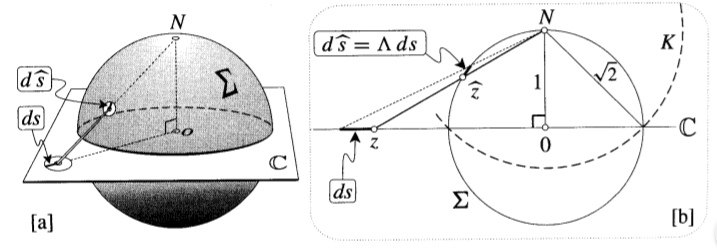
\includegraphics[scale=0.7]{fig_8}
        \label{fig_8}
    \end{figure}

    \item To compelete stereographic map we must find the associated metric function $\Lambda$ - that is ratio of the two radii as in figure. Recall that $[\td{a}\td{b}] = R^2[ab]/([qa][qb])$ so that $d\hat{s} = (2ds)/([Nz]^2) = (2ds)/(1+|z|^2)$. This flat conformal map (stereographic projection) with above metric is the desired depiction of all possible surfaces of constant Gaussian curvature $k=+1$.

    \item In general, suppose that $S$ is a surface of constant Gaussian curvature so that it posseses a group of motions and suppose that we have drawn a conformal map of $S$ with metric $d\hat{s} = \Lambda(z)ds$. Any motion of $S$ will induce a corresponding transformation of this map in $\C$. Since direct motions of the curved surface are conformal, the conformality of the map implies that the induced complex functions must also be conformal and hence analytic.
    
    \item Purely in terms of $\C$, we may therefore identify a function $f(z)$ as a motion if it is analytic and it "preserves the metric" $d\hat{s}=\Lambda(z)ds$. That is, suppose that the analytic function $z\mapsto \td{z}=f(z)$ sends two infinitesimally separated points $z$ and $z+dz$ to $\td{z}$ and $\td{z}+d\td{z}$. Then $f(z)$ is a motion iff the image separation $d\td{s}=|d\td{z}|$ on compelx plane is related to the original separation $ds=|dz|$ on complex plane by $\Lambda(\td{z})d\td{s} = \Lambda(z)ds$. Likewise, opposite motions of $S$ correspond to the anticonformal mappings of $\C$ that satisfy this equation.
    
    \item Since $d\td{z} = f'(z)dz$, this is equivalent to $f$ satisfying $|f'(z)| = \Lambda(z)/\Lambda(f(z))$.
    
    \item For the particular case $S=\Sigma$, and to the particular conformal map obtained by stereographic projection, the direct motions of all possible surfaces of constant Gaussian curvature $k=+1$ become set of analytic complex functions satisfying $|f'(z)| = (1+|f(z)|^2)/(1+|z|^2)$.

    \begin{figure}[h!]
        \centering
        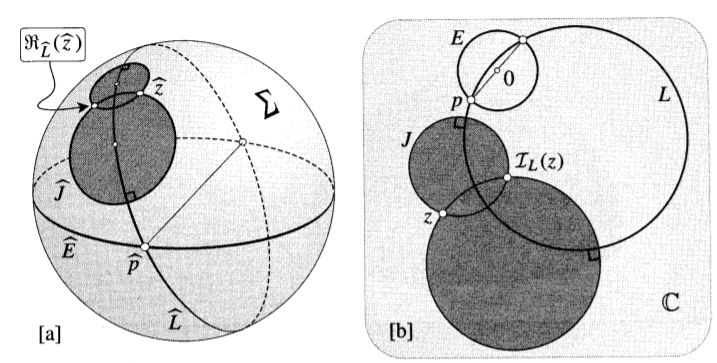
\includegraphics[scale=0.7]{fig_9}
        \label{fig_9}
    \end{figure}

    \item In principal, these functions can be found without ever leaving $\C$. However, it is simpler and more illuminating to return to the motions of $\Sigma$. Reflection of $\Sigma $ in a line induces reflection (inversion) of $\C$ in the stereographic image of that line. [Exercise 2]. $R^{\psi}_{\hat{a}} = \mc{R}_{\hat{L_2}} \circ \mc{R}_{\hat{L_1}}$ where $\hat{L_i}$ are any two circles passing through $\hat{a}$ and hence also through its antipodal points $\hat{b}$ s.t. angle between them is $\psi/2$. Since stereographic projection preserves circles and angles, the images in $\C$ of these two lines will be two circles passing through $a$ and $b=-1/\bar{a}$ and containing angle $\psi/2$. Therefore the transformation induced on $\C$ by above rotation on $\Sigma$ is $R_{a}^{\psi} = \mc{I}_{L_2} \circ \mc{I}_{L_1}$. This is a composition of two reflections (inversions) so is a non-loxodromic M.T.
    
    \begin{figure}[h!]
        \centering
        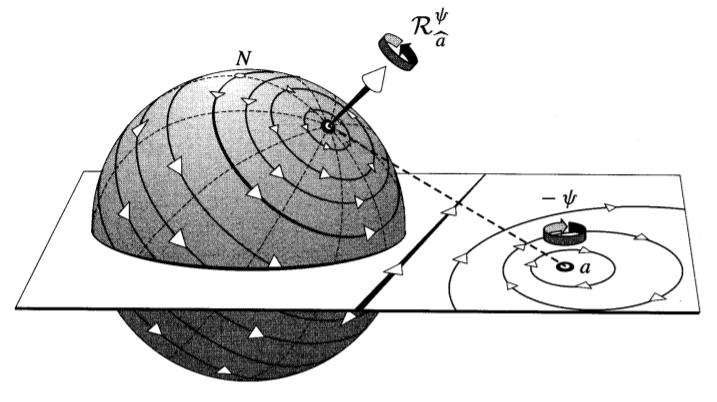
\includegraphics[scale=0.7]{fig_10}
        \label{fig_10}
    \end{figure}

    \begin{figure}[h!]
        \centering
        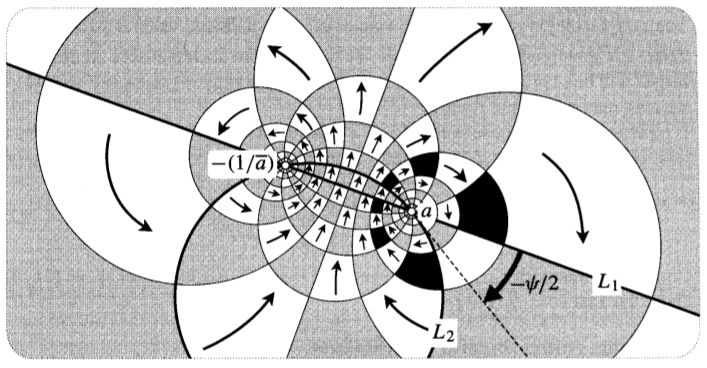
\includegraphics[scale=0.7]{fig_11}
        \label{fig_11}
    \end{figure}

    \item Since, multiplier describes local effect of a M.T. in the immediate neighbourhood of a fixed point, we have $m=e^{-i\psi}$ for the fixed point $a$ and $m=e^{i\psi}$ for the fixed point $-1/\bar{a}$.
    
    \item Using Exercise $4$ we have $R_{a}^{\psi}(z)$ is of form $(Az+B)/(-\bar{B}z+\bar{A})$. This formula represents the most general direct motion of $\Sigma$. More precisely,
    
    \begin{align*}
    [R^{\psi}_{a}] = \begin{bmatrix}e^{i(\psi/2)}|a|^2+e^{-i(\psi/2)} & 2ia\sin(\psi/2)\\2i\bar{a}\sin(\psi/2)& e^{-i(\psi/2)}|a|^2+e^{i(\psi/2)}\end{bmatrix}
    \end{align*}
    
    \item The most general opposite motion is represented by $z\mapsto (A\bar{z}+B)/(-\bar{B}\bar{z}+\bar{A})$ [Think of opposite motion as composition of three reflections. Then add two reflections (corresponding to $z\mapsto \bar{z}$) at the end which will not affect the overall output. Now, note that the first two reflections and next two reflections correspond to two rotations the composition which correspond to a single rotation].
    
    \item A new way to compute $R^{\omega}_{\hat{p}} \circ R^{\psi}_{\hat{a}}$ is by multiplying out the corresponsing $2\times 2$ matrices.
    
    \item We can also express the rotational transformation in terms of $\hat{a}$ rather than $a$ by transforming complex cartesian coordinates to spherical coordinates. If $\hat{a} \equiv (X,Y,Z)$ where $X^2+Y^2+Z^2=1$ then $a=(X+iY)/(1-Z)$ and $|a|^2 = (1+Z)/(1-Z)$. Substitute these values in above matrix to get,

    \begin{align*}
    [R^{\psi}_{V}] = \begin{bmatrix}\cos(\psi/2)+in\sin(\psi/2)&(-m+il)\sin(\psi/2)\\(m+il)\sin(\psi/2)&\cos(\psi/2)-in\sin(\psi/2)\end{bmatrix}
    \end{align*}

    \item No three dimensional analogue of complex numbers exist. Four-dimensional analogue is attainable. In two-dimensional complex plane, we may think fo $1$ and $i$ as unit basis "vectors" in terms of which a general complex number may be expressed as $z=a1+bi$. The algebra of $\C$ amounts to stipulating that multiplication distributes over addition, that $1$ is the identity and that $i^2=-1$.
    
    \item In four dimensional space, Hamilton introduced four basis vectors $1,I,J,K$ in terms of which a general vector $\V$ (which Hamilton called a quaternion) could be expressed as $\V = v1 + v_1I+v_2J+v_3K$ where the coefficients are all real numbers. To define the product of two such quarternions, Hamilton took $1$ to be the identity, and he took $I,J,K$ to be three different square roots of $-1$, each analogous to $i$: $I^2=J^2=K^2=-1$. As in ordinary algebra, Hamilton insistend that multiplication distribute over addition, but in order to render division possible, Hamilton postulated that $IJ=K=-JI$, $JK=I=-KJ$, $KI=J=-IK$ (Note that this is non-commutative multiplication).

    \item As in ordinary algebra, we suppress the identity $1$ and write $v1 = v$ which is the scalar part of $\V$. The reminaing term is $V = v_1Iv_2Jv_3K$ which is vector part of $\V$. Thus, $\V=v+V$. When $v$ vanishes, $\V$ is a pure quaternion. Multiplication of two quaternions yields, $\V\W = (vw-V.W) + (vW+wV+V\times W)$. When $v=0=w$, then $\V\W = -V.W + V\times W$.

    \item M.T. corresponding to binary rotation about the axis $v=li+mj+nk$ is $[R^{\pi}_{v}] = [in,-m+il;m+il,-in]$.

    \item Redefine $1 = [1,0;0,1]$, $I=[0,i;i,0]$, $J=[0,-1;1,0]$, $K=[i,0;0,-i]$. Corresponding M.T.s are $z, 1/z,-1/z,-z$. Note that all of these are binary rotation matrices, because the same transformation applied twice gives identity. Under matrix multiplication, these binary rotation matrices obey exactly the same laws as Hamilton's $1$,$I$,$J$,$K$. It follows that quaternion multiplication is equivalent to multiplying the corresponding $2\times 2$ matrices obtained by replacing $1,I,J,K$ with matrices above.

    \item Note that $[R^{\psi}_{v}] = \cos(\psi/2) + V\sin(\psi/2)$ where $V = lI + mJ + nK$. To compose two rotations of space, we need only multiply the corresponding quternions. For example- composition of rotation of $\pi/2$ about $i$ followed by a rotation of $\pi/2$ about $j$ - now becomes, $1/\sqrt{2}(1+J)1/\sqrt{2}(1+I) = 1/2(1+I+J-K)$ which is a rotation of $2\pi/3$ about $1/\sqrt{3}(i+j-k)$.

    \begin{figure}[h!]
        \centering
        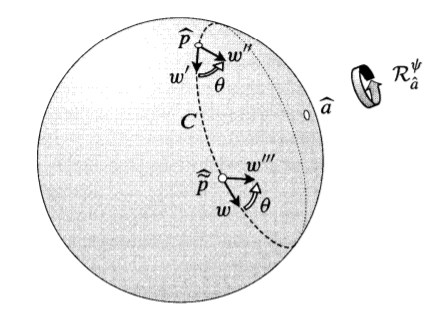
\includegraphics[scale=0.7]{fig_36}
        \label{fig_36}
    \end{figure}

    \item Effect of $R_{V}^{\psi}$ on position vector $P=Xi+Yj+Zk$: Suppose the result if $\td{P}$. Let us represent $P$ by the pure quaternion $\mb{P} = XI+YJ+ZK$, and likewise represent $\td{\mb{P}}$ as $\td{\mb{P}}$, then $\td{\mb{P}} = \R_{v}^{\psi}\mb{P}\R_{v}^{\psi}$.

\end{itemize}
\section{Hyperbolic Geometry}
\begin{itemize}
    \item A tractrix with radius of base $R$ has the following property: The segment of the tangent from the point of contact to the $Y$-axis has constant length $R$. Tractrix can also be constructed as an orthogonal trajectory through the family of circles of radius $R$ centred on the axis. [easy]

    \begin{figure}[h!]
        \centering
        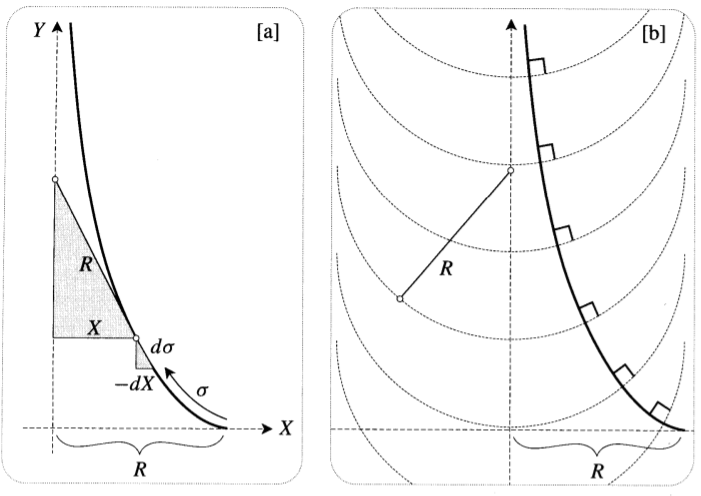
\includegraphics[scale=0.7]{fig_12}
        \label{fig_12}
    \end{figure}

    \item Let $\sigma$ represent arc length along the tractrix, with $\sigma=0$ corresponding to the starting position $X=R$. As from the figure, we have, $dX/d\sigma = -X/R$ i.e. $X=Re^{-\sigma/R}$.

    \item The pseudosphere of radius $R$ can be constructed as the surface obtained by rotating tractrix about its axis.

    \item [TODO] Geometric way to obtain constant negative curvature of Pseudosphere.

    \begin{figure}[h!]
        \centering
        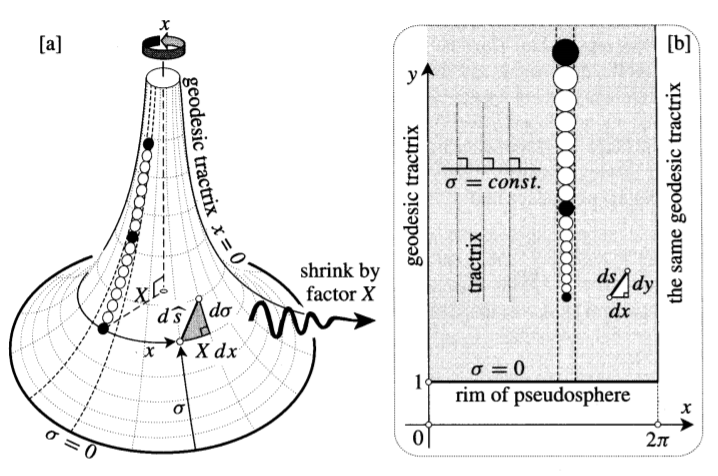
\includegraphics[scale=0.7]{fig_13}
        \label{fig_13}
    \end{figure}

    \item As in figure, $(x,\sigma)$ is a fairly natural coordinate system on pseudosphere, where $x$ measures the angle around the axis and $\sigma$ measures the arc length along each tractrix generator.
    
    \item Note that $x=$const. represents a tractrix generator which is a geodesic while $\sigma=$const. represents circular cross-section which is not a geodesic. Since radius of such a circle is same as $X$-coordinate, we have the radius $X$ of the circle $\sigma$=const. passing through the points $(x,\sigma)$ is given by $X=e^{-\sigma}$.

    \item Now, the first step is to find a conformal map of the pseudosphere. Let angle $x$ be our horizontal axis so that tractrix generators of the pseudosphere are represented by vertical lines. Let $(x,\sigma)$ on pseudosphere be represented by a point with Cartesian coordinates $(x,y)$. Here $y = y(x,\sigma)$. But our map needs to be conformal. Since tractrix generators ($x=$const.) and circular cross sections ($\sigma=$const.) are perpendicular to each other, their images in map must also be perpendicular. Since tractrix generators map to vertical lines, so circular cross sections must map to horizontal lines i.e. $y=$const. This means that $y$ is independent of $x$ i.e. $y=y(\sigma)$.
    
    \item Now, take a small vector emanating from $(x,\sigma)$ to $(x+dx,\sigma)$. These points subtend angle $dx$ at the centre of circular corss section so their separation on pseudosphere is $Xdx = e^{-\sigma}dx$. In the map, the two points lie on the horizontal line with a separation $dx$. So, the vector scales by $1/X$ going from pseudosphere to map. Since the map is conformal, every infinitsimal vector emenating from $(x,\sigma)$ on pseudosphere will undergo this scaling. So, we have the metric $d\hat{s} = Xds = e^{-\sigma}ds$.
    
    \item So a disc of radius $\epsilon$ will map to a disc of radius $\epsilon/X$. As the disc goes down the pseudosphere $X$ increases and so is itz size on the map decreases. Note that the angular width of the disc on pseudosphere is given by $\epsilon/X$ which has the same value as the size of the disc on the map.
    
    \item Finally, we have $dy=e^{\sigma}d\sigma$ so that $y=e^{\sigma}+c$ where we take $c=0$. So, pseudosphere is represented by the region above $y=1$ and the metric associated with the map is $d\hat{s}=Xds=ds/y = \sqrt{dx^2+dy^2}/y$. Also note that the apparent area $dxdy$ in the map is related to true area $dA$ on the pseudosphere by $dA=dxdy/y^2$.
    
    \item The abstract hyperbolic geometry was not interpreted as interinsic geometry of pseudosphere by Beltrami but was first discovered by Gauss, Bolyai and Lobachevsky, in a hyperbolic plane that is exactly like Euclidean plane except that lines within it obey hyperbolic axiom.

    \item The constant negative curvature of the pseudosphere ensures that it faithfully represents all consequences of this axiom that deal only with a finite region of the hyperbolic plane. An example of such a consequence is the theorem that $E(T)$ is negative multiple of $A(T)$ does indeed hold on the pseudosphere.

    \item Pseudosphere will not do as a model of the entire hyperbolic plane, because it departs from the Euclidean plane in two unacceptable ways:
    
    \begin{itemize}
        \item Pseudosphere is akin to a cylinder instead of a plane. For example, a closed loop in the plane can always be shrunk to a point, but a loop on the pseudosphere that wraps around the axis cannot. Beltrami pointed that this can be solved by imagining a thin stretchable sheet wrapped around pseudosphere infinitely many times, and as we unwrap (stretching as we go) we will the entire region above $y=1$. A particle travelling along a horizontal line in the map would correspond to a particle travelling round and round a circle $\sigma=$const. on the pseudosphere, executing one complete revolution for each movement of $2\pi$ along the line.

        \begin{figure}[h!]
            \centering
            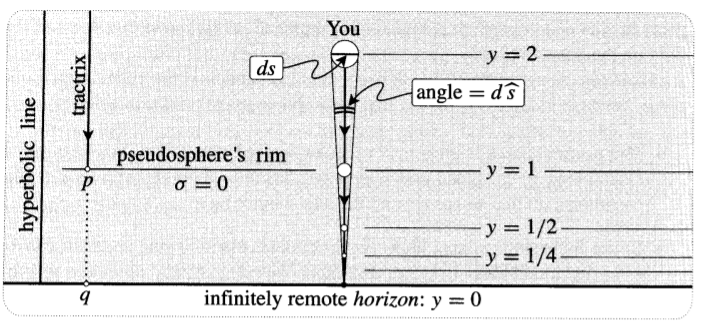
\includegraphics[scale=0.7]{fig_14}
            \label{fig_14}
        \end{figure}

        \item In the hyperbolic plane, as in the Euclidean plane, a line-segment can be extended indefinitely in either direction. Since tractrix generators of the pseudosphere are geodesic, we would like to interpret them as hyperbolic lines. But although such a tractrix extends indefinitely up the pseudosphere, in the other direction it terminates when it hits the rim. In terms of extrinsic geometry, the pseudosphere cannot be extended smoothly beyond this edge while preserving its constant curvature. However, intrinsic geometry is all we care about, so if we measure distance using $d\hat{s}=ds/y$ this is identical to the region $y>1$. As in figure, there is nothing preventing you to continue walking down to the point $q$ on $y=0$. Why stop at $q$? The answer is that you will never even get that far because $q$ is infinitely far from $p$. Suppose that you are the illustrated small disc on the line $y=2$, and that I am standing outside your hyperbolic world, watching as you walk at a steady pace towards $y=0$. Ofcourse you remain the same hyperbolic size as you walk, but to me you appear to shrink [because $ds = yd\hat{s}$]. The hyperbolic diameter of an infinitesimal disc centred at $(x+iy)$ is the angle it subtends at the point $x$ on the real axis. Thus your apparent size must shrink so that you subtend a constant angle, and although all your hyperbolic strides are the same legnth, to me they look shorter and shorter, and you appear to be travelling more and more slowly. For example, suppose you are walking at a steady spped of $\ln 2$. Integration of $dy/y$ shows that you reach $y=1$ after one unit of time, $y=1/2$ after two units of time, $y=1/4$ after three units of time, etc. Thus, viewed from outside your world, each successive unit of time only halves your distance from $y=0$, and therefore you will never reach it. [This is "Zeno's Revenge"].
    \end{itemize}

    \item Hyperbolic plane is the entire shaded half-plane $y>0$ with metric $d\hat{s}=ds/y$. The points on the real axis are infinitely far drom ordinary points and are not (strictly speaking) considered part of the hyperbolic plane. They are called ideal points, or points at infinity. The complete line $y=0$ of points at infinity will be called the horizon.

    \item Still it would be good to have a surface that is isometric (one-to-one mapping) to the entire hyperbolic plane. Hilbert proved that every pseudospherical surface necessarily has an edge beyond which it cannot be smoothly extended while preserving its constant negative curvature. Thus the upper half-plane with metric $d\hat{s}=ds/y$ is as good a depiction of the hyperbolic plane as we are going to get. Good thing is: there exist different types of maps to represent the hyperbolic plane: Poincare upper half-plane, Poincare disc, Klein disc. Note that Beltrami obtained all these models from a fourth model consisting of a map drawn on a hemisphere (which was also Beltrami's model).

    \item Multitude of parallel lines i =n the hyperbolic plane yields a geometry that is richer than Euclid's, containing rotations, translations, and a third kind of motion that has no Euclidean counterpart.

    \item $\mc{H}\{z_1,z_2\}$ be the $h$-distance (measured using $d\hat{s}=ds/y$) between $z_1$ and $z_2$. If $dz$ is infinitesimal, then $\mc{H}\{z+dz,z\} = |dz|/\mf{Im}z$. $h$-circle of $h$-radius $\rho$ and $h$-centre $c$ is the locus of points $z$ s.t. $\mc{H}\{z,c\} = \rho$.

    \begin{figure}[h!]
        \centering
        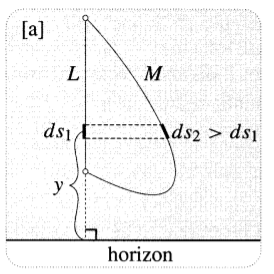
\includegraphics[scale=0.7]{fig_15}
        \label{fig_15}
    \end{figure}

    \item Since tractrix generators of the pseudosphere are clearly geodesic, vertical lines in the map should also be geodesic i.e. they should be example of $h$-lines i.e. The unique shortest route between two vertically separated points is the vertical line-segment $L$ connecting them. As in figure, $d\hat{s}_1 = ds_1/y < ds_2/y = d\hat{s}_2$, the total hyperbolic length of $L$ is less than $M$'s.

    \item So, we have $\mc{H}\{x+iy_1,x+iy-2\} = \int_{x+iy_1}^{x+iy_2}|dz|/\mf{Im}z = \int_{y_1}^{y_2}dy/y = |\ln(y_1/y_2)|$. Note that the integration depends on path corresponding to shortest route which, here, is straight vertical line.

    \item Through a given point of the pseudosphere we obviously have geodesics in all direction, not just tractrix generators. Every $h$-line is either a half-line orthogonal to the horizon, or else a semicircle orthogonal to the horizon. Note that if you were a habitant of the hyperbolic plane (say you are on a pseudosphere), there would be no way for you to distingushi between semicircular $h$-lines and the vertical $h$-lines (because intrinsic geometry is same everywhere). Also note that both semicircle and vertical h-lines have two ends. Former having both on the horizon, while later having one on horizon and one at $\infty$ (as we move upward along two vertical $h$-lines, the $h$-distance between them dies away like $1/y$ and they converge to a single point (this can be seen on pseudosphere)). Also, vertical $h$-lines can be viewed as just a special cse of a semicircular $h$-line by allowing the radius tend to $\infty$. We will prove the above fact about $h$-lines by first proving that inversion in a semicircle orthogonal to the horizon is an opposite motion of the hyperbolic plane.

    \begin{figure}[h!]
        \centering
        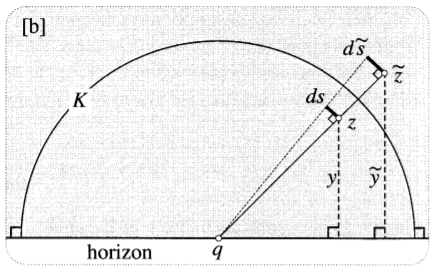
\includegraphics[scale=0.7]{fig_16}
        \label{fig_16}
    \end{figure}

    \item Since our hyperbolic model is conformal, we need only show that $\mc{I}_{K}(z)$ preserves the $h$-length of any single $ds$, in a direction of our choosing. As in figure, by similarity of triangles, $d\hat{\td{s}} = d\td{s}/\td{y} = ds/y = d\hat{s}$.

    \begin{figure}[h!]
        \centering
        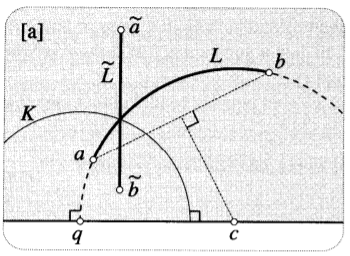
\includegraphics[scale=0.7]{fig_17}
        \label{fig_17}
    \end{figure}

    \item Now taking two arbitrary points $a$ and $b$ s.t. $\mf{Re}(a)\neq \mf{R}(b)$, one can always find a unique semicircle centred at origin passing through these two points (draw perpendicular bisector of $ab$ and find intersection of it with horizon). As in figure, we need to show that $L$ is the shortest route (has smallest $h$-length) from $a$ to $b$.

    \item Consider inversion of $L$ in a semicircle centred at $q$ (of any radius). Then $L$ will have vertical line segment as image. If $L$ is not the shortest route from $a$ to $b$ (say $M$ is the one) then $\td{M}$ will have smaller $h$-length than $\td{L}$. But as we showed before, this is not possible, so, $L$ is indeed shortest route from $a$ to $b$. Also, $\mc{H}\{a,b\} = \mc{H}\{\td{a},\td{b}\} = |\ln(\mf{Im}(\td{a})/\mf{Im}(\td{b}))$. So, semicircle orthogonal to horizon is an $h$-line. So, we have, inversion in a semicircle $K$ orthogonal to the horizon is a reflection $\Re_{K}$ of the hyperbolic plane in the $h$-line $K$. So, $\Re_{K}(z) = \mc{I}_{K}(z)$.

    \begin{figure}[h!]
        \centering
        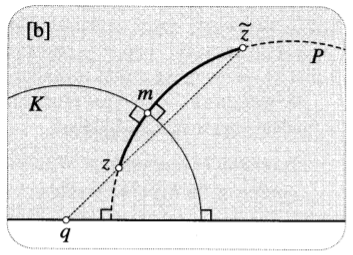
\includegraphics[scale=0.7]{fig_18}
        \label{fig_18}
    \end{figure}

    \item To prove this first understand what we mean by reflection. As in EG and SG, we begin by drawing $h$-line $P$ that passes through $z$ and cuts $K$ perpendicularly, say at $m$. Then, $\Re_{K}(z)$ is defined to be the point on $P$ that is the same $h$-distance from $m$ as $z$. Now as in figure, note that every semicircle through $z$ and $\td{z}$ will be orthogonal to $K$. The unique $h$-line through $z$ and $\td{z}$ will thus be perpendicular to $K$ and is the desired $P$. Now, note that inversion in $K$ maps $P$ to itself, swapping the segments $zm$ and $\td{z}m$. Since $\mc{I}_K$ is a motion, the two $h$-line segments have equal $h$-lengths.

    \item Conversely, if we are given any two points $z$ and $\td{z}$, then we may draw the perpendicular $h$-bisector $K$, and $\Re_{K}$ swaps $z$ and $\td{z}$. Also, note that $z$ and its reflection $\td{z}=\Re_{K}(z)$ are the same $h$-distance from every point $k$ on $K$, just as in EG and SG. Proof: Since $\mc{I}_K$ is a motion, and $\td{k} = \mc{I}_{K}(k)=k$, it follows that $\mc{H}\{z,k\} = \mc{H}\{\td{z},\td{k}\} = \mc{H}\{\td{z},k\}$.

    \begin{figure}[h!]
        \centering
        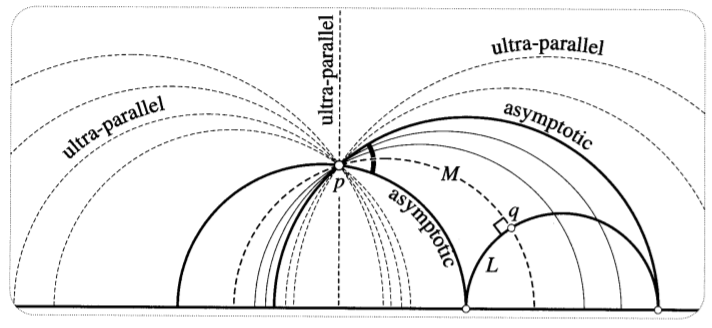
\includegraphics[scale=0.7]{fig_19}
        \label{fig_19}
    \end{figure}
    
    \item As in figure, there are infinitely many $h$-lines through $p$ that do not intersect $L$. Such $h$-lines are called ultra-parallel to $L$. Asymptotic $h$-lines fail to meet $L$ anywhere within the hyperbolic plane proper except at a point on horizon.

    \item As in EG, there is precisely one $h$-lin $M$ passing through $p$ that cuts $L$ at right angles (say at $q$). In fact, $M$ may be constructed as the unique $h$-line through $p$ and $\Re_{L}(p)$ ($h$-line passing through $p$ and perpendicular to $L$ must pass through $\Re_{L}(p)$. Note that there is a unique $h$-line passing through two arbitrary points). The existence of $M$ makes it possible to define the distance of a point $p$ from a line $L$, as the $h$-length of the segment $pq$ of $M$.

    \item Since $M$ and $L$ are orthogonal, $\Re_{M} = \mc{I}_M$ maps $L$ into itself, swapping the two ends on the horizon. It follows that $\Re_{M}$ swaps the two asymptotic lines, and that $M$ bisects the angle at $p$ contained by the asymptotic lines. The angle between $M$ and either asymptotic line is called the angle of parallelism, and is usually denoted by $\prod$. As one rotates the line $M$ about $p$, its intersection point $L$ moves off towards infinity, and $\prod$ tells you how far you can rotate $M$ before it starts missing $L$ entirely.

    \begin{figure}[h!]
        \centering
        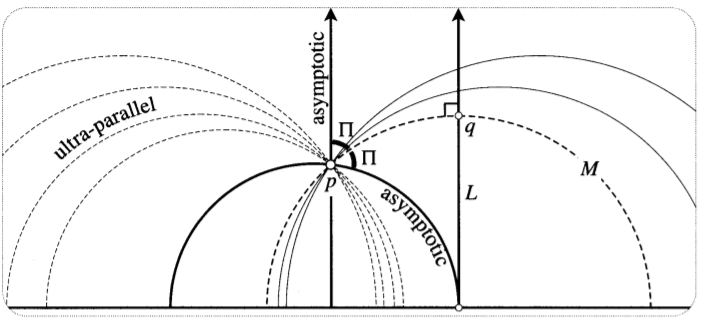
\includegraphics[scale=0.7]{fig_20}
        \label{fig_20}
    \end{figure}

    \item Following figure illustrate the same concepts for the case when $h$-line $L$ is vertical.

    \item [TODO] finding angle of parallelism.

    \item If $L_1$ and $L_2$ are two $h$-lines, then the composition, $\mc{M}\equiv \Re_{L_2} \circ \Re_{L_1}$ of $h$-reflection in these lines will be a direct motion of the hyperbolic plane. Since $h$-reflection is inversion in a circle, we have $\mc{M}$ is a non-loxodromic M.T. (we will prove that every direct motion is represented as a (non-loxodromic) M.T.).

    \item Conversely, suppose that $M(z)$ is an arbitrary M.T. that maps the upper half-plane to itself. Then $M(z)$ must map the real axis into itself. But loxodromic M.T> cannot possess such an invariant line. Thus $M(z)$ is non-loxodromic and is thus composition of inversion in two circles orthogonal to the real axis. Thus the most general M.T. of the upper half plane to itself represents a direct hyperbolic motion of teh type $\mc{M}$ above. One way to discover algebraic form of $\mc{M}$ is composition of two inversions. Another way is a direct approach. Both gives $M(z) = (az+b)/(cz+d)$ where $a,b,c,d\in\R$ and $(ad-bc) > 0$.

    \item $\mc{M} \equiv \Re_{L_1} \circ \Re_{L_2}$ is one of the three fundamentally different types:
    
    \begin{itemize}
        \item If the $h$-lines intersect, then $\mc{M}$ is (of type elliptic) called a hyperbolic rotation.

        \item If the $h$-lines are asymptotic, then $\mc{M}$ is (of type parabolic) a new kind of motion (peculiar to hyperbolic geometry) called a limit rotation.

        \item If the $h$-lines are ultra-parallel, then $\mc{M}$ is (of type hyperbolic) called a hyperbolic translation.
    \end{itemize}

    \begin{figure}[h!]
        \centering
        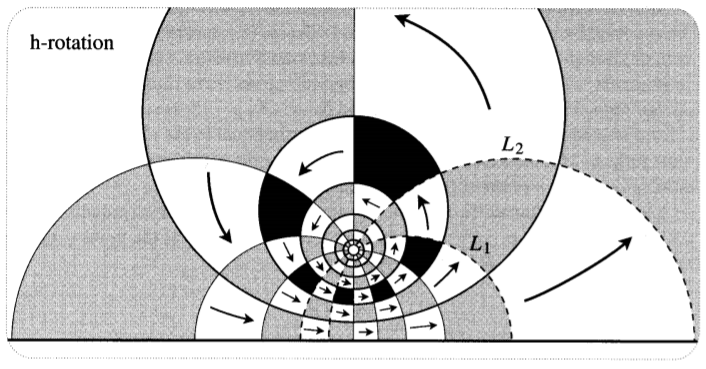
\includegraphics[scale=0.7]{fig_21}
        \label{fig_21}
    \end{figure}

    \item When $L_1$ and $L_2$ intersect at $a$ such that the angle from $L_1$ to $L_2$ is $(\phi/2)$ - this gives rise to $\mc{R}_{a}^{\phi}$ which has fixed points $a$ and $\bar{a}$ and the multiplier associated with $a$ is $m=e^{i\phi}$. Effect of $\mc{R}_{a}^{\phi}$ on an infinitesimal neighbourhood of $a$ is just a Euclidean rotation of $\phi$ about $a$. But since the map is conformal, this implies that a Poincarite standing at $a$ will also see his immediate neighbourhood undergoing a rotation of $\phi$. As a matter of fact, the Poincarite at $a$ will see the entire hyperbolic plane undergoing a perfect rotation of $\phi$. Every $h$-line segment $ap$ emanating from $a$ is transformaed into another $h$-line segment $a\td{p}$ of equal length, making angle $\phi$ with the original. If $\phi$ is increased from $0$ to $2\pi$, then $\td{p}$ traces a $h$-circle centred at $a$, while in the map we see $\td{p}$ miraculously tracing out a Euclidean circle. \tt{Every $h$-circle is represented in the map by a Euclidean circle, and its $h$-centre is the intersection of any two $h$-lines orthogonal to it. Algebraically, the $h$-circle with $h$-centre $a=x+iy$ and $h$-radius $\rho$ is represented by the Euclidean circle with centre $(x+iy\cosh \rho)$ and radius $y\sinh \rho$} [very simple solution].

    \begin{figure}[h!]
        \centering
        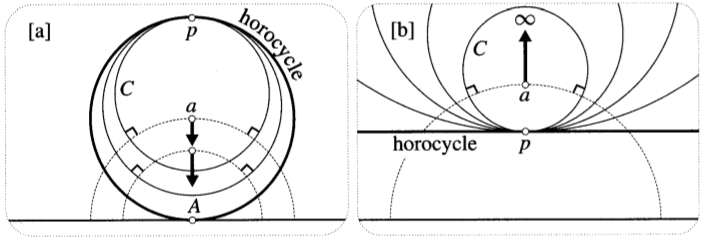
\includegraphics[scale=0.7]{fig_22}
        \label{fig_22}
    \end{figure}

    \item In EG, suppose there is a line $L$, a fixed point $p$ on it and a movable point $a$ on it. Suppose there is a circle centred at $a$ passing through $p$. As $a$ approaches $\infty$ from either side, the circle becomes a straight line $\perp$ to $L$ passing through $p$. This is true irrespective of the orientation of $L$. In contrast in hyperbolic plane, as $a$ moves towards infinitely remote point $A$ on the real axis, the limiting form of $C$ is a (Euclidean) circle that touches the real axis at $A$. This is neither an ordinary $h$-circle (distance of every point inside it from $A$ is $\infty$ while from any other point is a finite value) nor an $h$-line: it is a new type of curve called a horocycle. If we invert this circle in an $h$-line centred at $A$ then we will get a horizontal (Euclidean) line. Poincarites cannot distingush between the two types of curves so the later horizontal (Euclidean) lines are also horocycles.

    \begin{figure}[h!]
        \centering
        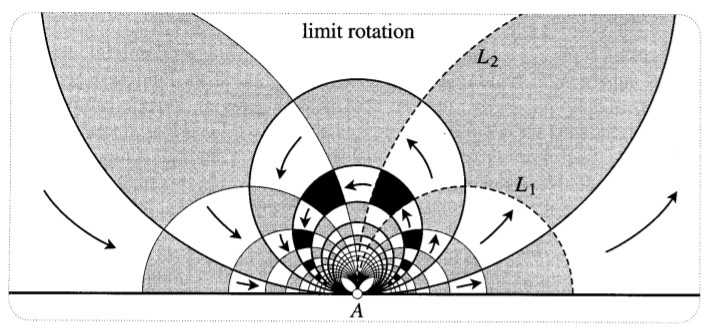
\includegraphics[scale=0.7]{fig_23}
        \label{fig_23}
    \end{figure}

    \item As in figure, $h$-reflection in $h$-lines $L_1$ and $L_2$ that are asymptotic at $A$ results in limit-rotation ($h$-rotation $\mc{R}_{a}^{\phi}$ where $a$ tends to $A$ on horizon). Invariant curves are horocycles touching at $A$; each horozycle is orthogonal to every $h$-line that ends at $A$; and any two such horocycles cut off the same $h$-length on every $h$-line that ends at $A$ ($h$-length is $\infty$ because other end is at $A$ which is on horizon). When asymptotic $L_1$ and $L_2$ are vertical Euclidean half-lines, say separated by $\alpha/2$, then $\mc{M} = \Re_{L_2}\circ\Re_{L_1}$ is represented by composition of two Euclidean reflections in parallel lines. Thus $\mc{M}$ is a Euclidean translation $z\mapsto z+\alpha$ of the upper half-plane, and invariant curves are horizontal lines, which are again horocycles. Note that this Euclidean translation is not an $h$-translation, which becomes clear on pseudosphere where this translation becomes rotation through angle $\alpha$ about its axis.

    \begin{figure}[h!]
        \centering
        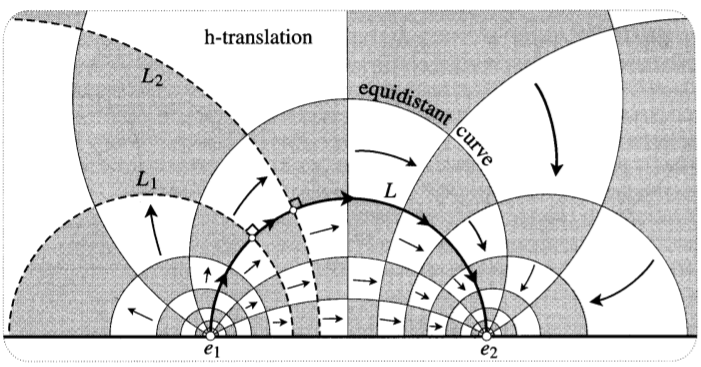
\includegraphics[scale=0.7]{fig_24}
        \label{fig_24}
    \end{figure}

    \item When two $h$-lines are ultra-parallel, we get $h$-translation. Note that there is precisely one $h$-line $L$ that is orthogonal to both $L_1$ and $L_2$. Unlike a Euclidean translation where infinitely many $h$-lines map into itself, in $h$-translation, $L$ is the only $h$-lines that is mapped into itself. It is called the axis of $h$-translation. Every point on the $h$-lines is moved by the same $h$-distance $\delta$ along $L$ (that's why the name $h$-translation). If we assume that axis $L$ has a direction assigned to it, then we may unambiguously denote this $h$-translation by $\mc{T}_{L}^{\delta}$. Unlike EG where invariant curves of translation are parallel lines, in $h$-translation, invariant curves of $\mc{T}_{L}^{\delta}$ are not $h$-lines but rather arcs of Euclidean circles connecting ends $e_1$ and $e_2$ of $L$. These are called equidistant curves of $L$, because every point on such a curve is the same $h$-distance from the $h$-line $L$ [To see this, take a point $p$ on $L$ and the corresponding shortest route point $p'$ on an equidistant curve $L'$. By varying $\delta$ one can map $p$ to any arbitrary point $q$ on $L$ and because of conformality of $\mc{T}_{L}^{\delta}$, $p'$ will be mapped to the corresponding shortest route point from $q$, on $L'$ i.e. $q'$. Since $\mc{T}_{L}^{\delta}$ preserves distance, we have, the distance of every point on $L'$ from $L$ is equal]. When $L_1$ and $L_2$ are represented by ultra-parallel concentric Euclidean semicircles, say centred at the origin, then, two $h$-reflections yield a central dilation $z\mapsto kz$, where $k$ is a real expansion factor. The axis of this $h$-translation is the vertical line through the origin (the $y$-axis), and the equidistant curves are all other (Euclidean) lines through the origin. Note that this Euclidean expansion is a similarity transformation of the map, but it is not a similarity transformation of the hyperbolic plane.

    \item Note that Poincarites can distinguish between these three types of direction motions. For example, only $h$-rotation have invariant circles, and only $h$-translations have an invariant $h$-line.

    \item [TODO] Showing that every direct motion can be classified into one of three types above.

    \item $A(\text{pseudosphere}) = \int_{0}^{2\pi}\int_{1}^{\infty}dydx/y^2 = \int_{0}^{2\pi}dx\int_{1}^{\infty}dy/y^2 = 2\pi$.

    \begin{figure}[h!]
        \centering
        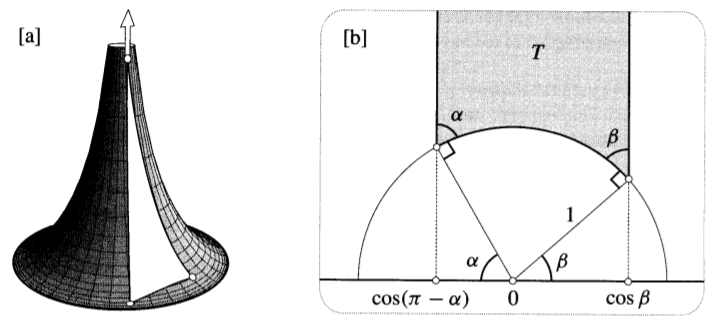
\includegraphics[scale=0.7]{fig_25}
        \label{fig_25}
    \end{figure}

    \item For a triangle on a pseudosphere, if the uppermost vertex moves up the pseudosphere indefinitely, then the angle at the vertex tends to zero, and the edges meeting at that vertex tend to asymptotic lines, namely, tractrix generators meeting at $\infty$. Such a limiting triangle, two of whose edges are asymptotic, is called an asymptotic triangle. As in figure, without loss of generality we can assume the circle to be unit circle (if the arc is on circle of radius $r$ centred at $x=X$ then it can be transformed to arc on unit circle by limit rotation $z\mapsto z-X$ and $h$-translation $x\mapsto z/r$, both of which would preserve the $h$-length of triangle and thus the area of the corresponding triangle on pseudosphere). We have,
    
    \begin{align*}
        A(T) &= \int_{\cos(\pi-\alpha)}^{\cos\beta}(\int_{\sqrt{1-x^2}}^{\infty}dy/y^2)dx\\
        &= \int_{\cos(\pi-\alpha)}^{\cos\beta} 1/(\sqrt{1-x^2})dx\\
        &= \pi-\alpha-\beta
    \end{align*}

    \begin{figure}[h!]
        \centering
        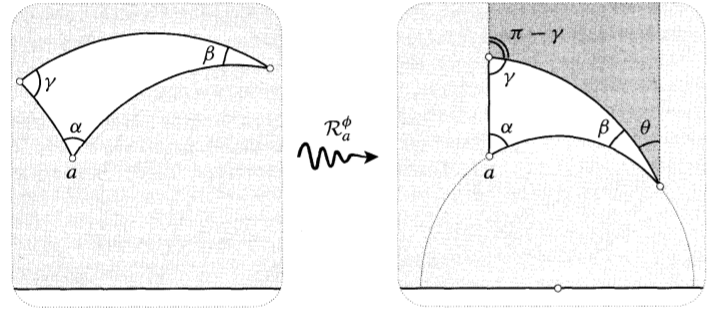
\includegraphics[scale=0.7]{fig_26}
        \label{fig_26}
    \end{figure}

    \item Now for a general triangle, we first apply a suitable $h$-rotation about one of the vertices so that one of the edge becomes vertical. Then, following figure, we have $A(T) = \pi-\alpha-(\beta+\theta)-(\pi-(\pi-\gamma)-\theta)=\pi-\alpha-\beta-\gamma = -E(T)$

    \item Another useful conformal map of hyperbolic plane is Poincare disc which maps entire upper half-plane into unit disc by: $z \mapsto \mc{I}_{K}(z)$ followed by $z\mapsto \bar{z}$ (which makes it a conformal map) where $K$ is as shown in the figure. In order for the disc to represent the hyperbolic plane, its metric must be inherited from the upper half-plane. That is, we must defined $h$-separation $\mc{H}\{\td{a},\td{b}\}$ of two points in the disc to be the $h$-separation $\mc{H}\{a,b\}$ of their preimages in the upper half-plane. This implies that the $h$-lines of the disc are precisely the images of $h$-lines in the upper half-plane. As in the figure, with $\mc{I}_{K}(z)$,

    \begin{figure}[h!]
        \centering
        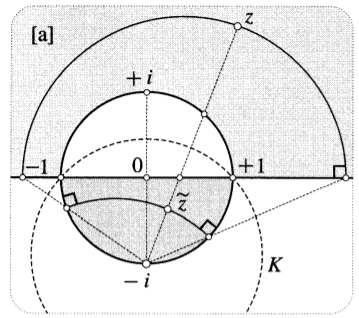
\includegraphics[scale=0.7]{fig_27}
        \label{fig_27}
    \end{figure}

    \begin{itemize}
        \item $\pm 1$ remains fixed and $i$ is mapped to $0$.

        \item Entire shaded part of the upper half-plane is mapped to the shaded bottom half of the unit disc.

        \item Reimaing part of the upper half-plane (i.e. top half of the unit disc) is mapped into itself.

        \item $h$-lines in the disc are the images of $h$-lines in the upper half-plane, and these are arcs of circles orthogonal to the unit circle.
        
        \item The entire horizon of the hyperbolic plane is represented by the unit circle, with common point at $\infty$ of vertical $h$-lines in the upper half-plane being represented by $-i$.
    \end{itemize}

    \item The net transformation from Poincare upper half-plane to the Poincare disc is thus a M.T. say $D(z)$. Since $D(i)= 0$ and $D(-i)=\infty$ so $D(z) = k(z-i)/(z+i)$. Also, $D(\pm 1) = \pm 1$ so that $D(z) = (iz+1)/(z+i)$.

    \item Horizon is also called circle at infinity because it is mapped to the unit circle.

    \begin{figure}[h!]
        \centering
        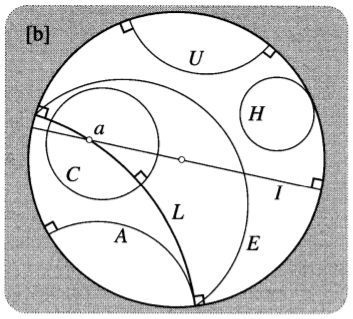
\includegraphics[scale=0.7]{fig_28}
        \label{fig_28}
    \end{figure}

    \item As in figure, $I$ intersects $L$, $A$ is asymptotic to $L$ and $U$ is ultra-parallel to $L$. Euclidean circle $C$ lying inside $D$ represents $h$-circle though its $h$-centre $a$ does not generally coincide with its Euclidean centre. Horocycles in $D$ are represented by circles such as $H$ that touch the unit circle.

    \begin{figure}[h!]
        \centering
        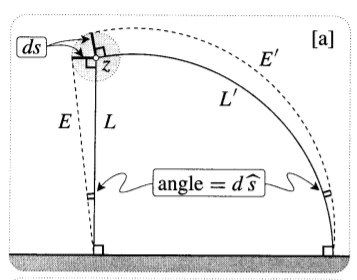
\includegraphics[scale=0.7]{fig_29}
        \label{fig_29}
    \end{figure}

    \item As in figure, recall that if $ds$ is the infinitesimal Euclidean length of a horizontal line-element emanating from $z$, then the angle between $L$ and $E$ is its hyperbolic length $d\hat{s} = [ds/\mf{Im}(z)]$. Note that in purely hyperbolic terms, $L$ is an $h$-line orthogonal to $ds$, and $E$ is an equidistant curve of $L$. If we apply an $h$-rotation $\mc{R}^{\phi}_{z}$ then $L$ is carried into another $h$-line $L'$, and $E$ is carried into an equidistant curve $E'$ of $L'$, and the angle between $L'$ and $E'$ is the same as before.
    
    \item Through one end of $ds$, draw the $h$-line $l$ orthogonal to $ds$, and through the other end of $ds$ draw the equidistant curve $e$. Then the $h$-length $d\hat{s}$ of $ds$ is the angle of intersection (on the horizon) of $l$ and $e$.

    \item Since M.T. $D$ to the Poincare disc is conformal, so the above construction of $d\hat{s}$ is valid there too.

    \begin{figure}[h!]
        \centering
        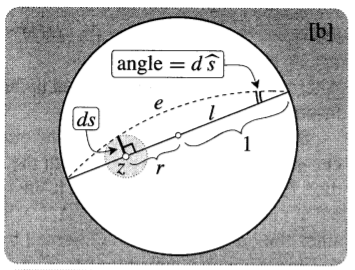
\includegraphics[scale=0.7]{fig_30}
        \label{fig_30}
    \end{figure}

    \item Because the map is conformal, the $h$-length $d\hat{s}$ of $ds$ is independent of the direction of $ds$, so we may simplify the construction by choosing $ds$ orthogonal to the diameter $l$ through $z$. Then $e$ is the equidistant curve which is an arc of a Euclidean circle through the ends of $l$. If $\rho$ is the radius of the circle containing the arc $e$, then, $1 = \rho d\hat{s}$.

    \begin{figure}[h!]
        \centering
        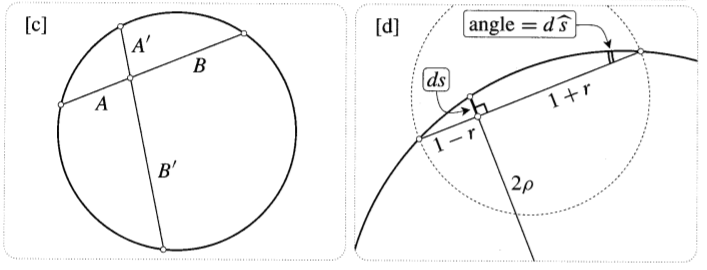
\includegraphics[scale=0.7]{fig_31}
        \label{fig_31}
    \end{figure}

    \item Using the property that all chords passing through a fixed interior point are divided into two parts whose length have constant product: $AB = A'B'$, we get, $2\rho ds = (1-r)(1+r)$ where $r=|z|$. Thus metric of Poincare disc is,

    \begin{align*}
        d\hat{s} = 2ds/(1-|z|^2)
    \end{align*}

    Since the Euclidean line-segment connecting $0$ to $z$ is also an $h$-line segment, we can now find the $h$-separation os these points as follows:

    \begin{align*}
        \mc{H}\{0,z\} = \int_{0}^{|z|}2dr/(1-r^2) = \ln((1+|z|)/(1-|z|))
    \end{align*}

    \item Note that as $z$ moves towards the unit circle (the horizon), $\mc{H}\{0,z\}$ tends to infinity, as it should.

    \item Since the intrinsic geometry of the Poincare disc is identical to the upper half-plane, every direct motion in the Poincare disc is composition of two $h$-reflections. In the upper half-plane $h$-reflection in an $h$-line $K$ meant geometric inversion in $K$, and the same is true in the Poincare disc. Suppose $q$ is the $h$-reflection of $p$ in $K$. Since $D(z)$ preserve the hyperbolic distance (i.e. the $h$-distance between two points and the image points are same) and $D(z)$ is M.T., so, by symmetry principle, $\td{p}$ and $\td{q}$ are summetric about $\td{K}$. Thus every direct motion $\mc{M}$ of the Poincare disc has form $\mc{M} = \Re_{L_2} \circ \Re_{L_1} = \mc{I}_{L_2} \circ \mc{I}_{L_1}$ where $L_1$ and $L_2$ are $h$-lines, namely, arcs of circles orthogonal to the unit circle.

    \item As in the upper half-plane, ever direct motion of Poincare disc is a non-loxodromic M.T. We get $h$-rotations when $L_1$ and $L_2$ intersect, a limit rotation when they are asymptotic, and an $h$-translation when they are ultra-parallel. Following figures will help visualize these. Infer the parallels between these and direct motions in upper half-plane.

    \begin{figure}[h!]
        \centering
        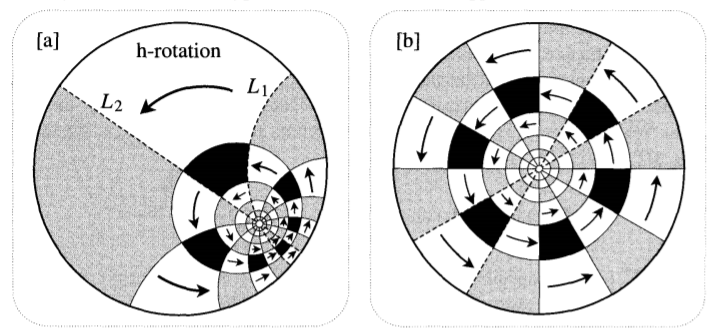
\includegraphics[scale=0.7]{fig_32}
        \label{fig_32}
    \end{figure}

    \begin{figure}[h!]
        \centering
        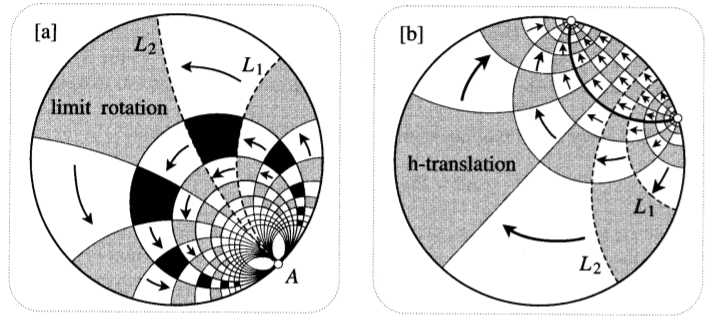
\includegraphics[scale=0.7]{fig_33}
        \label{fig_33}
    \end{figure}

    \item Every direct motion is a Mobius transformation mapping unit disc to itself i.e. M.A. of the unit disc. The formula representing most general M.A. is $M_{a}^{\phi} = e^{i\phi}M_{a}(z)$ where $M_{a}(z) = (z-a)/(\bar{a}z-1)$. Recall that $M_a = \mc{I}_B \circ \mc{I}_a$ where $B$ is the diameter through $a$ and where $A$ is the circle centred at $(1/\bar{a})$ that is orthogonal to the unit circle.

    \begin{figure}[h!]
        \centering
        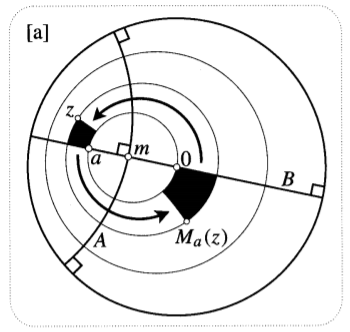
\includegraphics[scale=0.7]{fig_34}
        \label{fig_34}
    \end{figure}

    \item Hyperbolic geometry gives us a fresh perspective on this result: the intersection point $m$ of $A$ and $B$ is the $h$-midpoint of $0$ and $a$ [because $M_a$ is a motion (so preserves distances) and it swaps $0$ and $a$ about $m$ so that $\mc{H}\{0,m\} = \mc{H}\{m,a\}$], and $A$ itself is the perpendicular $h$-bisector of $0a$. Furthermore, the ivnersions in $A$ and $B$ are $h$-reflections. Thus $M_a$ is the composition of two $h$-reflections in perpendicular $h$-lines through $m$, and so \tt{The unique M.A. $M_a$ that swaps $a$ and $0$ is the $h$-rotation $\mc{R}^{\pi}_{m}$ through angle $\pi$ about the $h$-midpoint $m$ of the $h$-line segment $0a$}.

    \item We can now easily find the formula for $h$-separation of any two points, $a$ and $z$. The $h$-rotation brings $a$ to the origin, so,

    \begin{align*}
        \mc{H}\{a,z\} &= \mc{H}\{M_a(a),M_a(z)\}\\
        &= \mc{H}\{0, M_a(z)\}\\
        &= \ln((1+|M_a(z)|)/(1-|M_a(z)|))\\
        &= \ln((|\bar{a}z-1|+|z-a|)/(|\bar{a}z-1|-|z-a|))
    \end{align*}

    \item The Euclidean rotation $z\mapsto e^{i\phi}z$ represents the $h$-rotation $\mc{R}^{\phi}_{0}$. Thus the most general M.A. of the disc may be interpreted as composition of two $h$-rotations: $M_a^{\phi} = \mc{R}_0^{\phi} \circ \mc{R}_{m}^{pi}$.

    \item Figure shows how the two $h$-rotations can be composed. The $h$-rotation $\mc{R}^{\phi}_{0}$ is the composition of $h$-reflections in any two $h$-lines through $0$ (diameters) containing angle $\phi/2$. Thus choosing first $h$-line to be $B$ and second to be $C$, we get, $M_{a}^{\phi} = (\Re_{C}\circ \Re_{B}) \circ (\Re_{B} \circ \Re_{A}) = \Re_{C} \circ \Re_{A}$. Thus $M_a^{\phi}$ is an $h$-rotation, limit rotation or $h$-translation according as $A$ and $C$ are intersecting, asymptotic or ultra-parallel.

    \begin{figure}[h!]
        \centering
        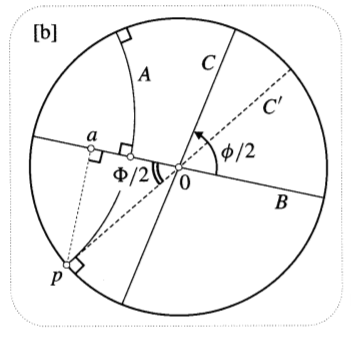
\includegraphics[scale=0.7]{fig_35}
        \label{fig_35}
    \end{figure}

    \item Thinking of $a$ as fixed and $\phi$ as variable, the critical value $\phi=\Phi$ separating the $h$-rotations from the $h$-transltions occurs when $C$ is in the position $C'$ asymptotic to $A$ at $p$. Since $pa0$ is right angled, we have $\Phi = 2\cos^{-1}|a|$. Thus we have shown: the most general M.A. $M_a^{\phi}$ of the disc is a direct hyperbolic motion, and it is $(i)$ and $h$-rotation if $\phi<\Phi$; $(ii)$ a limit rotation if $\phi=\Phi$; and $(iii)$ an $h$-translation if $\phi>\Phi$. Recall that the set of M.T. of form $M_a^{\phi}$ is identical to the set of form $(Az+B)/(\bar{B}z+\bar{A})$ where $|A|>|B|$.
\end{itemize}

\section{The Hemisphere Model and Hyperbolic Space}
\end{document}